\documentclass{article} % Tipo de documento
\usepackage[utf8]{inputenc} % Permite el uso de caracteres del Español
\usepackage[T1]{fontenc}
\usepackage{hyperref}
\usepackage{graphicx}
\usepackage{wrapfig}
\usepackage{subcaption}
\newcommand{\grad}{$^{\circ}$}

% set font encoding for PDFLaTeX or XeLaTeX
\usepackage{ifxetex}
\ifxetex
  \usepackage{fontspec}
\else
  \usepackage[T1]{fontenc}
  \usepackage[utf8]{inputenc}
  \usepackage{lmodern}
\fi

% used in maketitle
\title{Reporte Actividad 2: Introducción a Python, Jupyter y Pandas}
\author{Melissa Matrecitos Avila}
\date{07 de Febrero de 2018}

\begin{document}
\maketitle
\section{Introducción}

\begin{wrapfigure} {l}{0.35\textwidth}
  \centering
  
\includegraphics[width=0.2\textwidth]{Python.png}
  \caption{Logo de Python}
  \label{fig:Logo}
\end{wrapfigure}

El siguiente texto es el reporte de la actividad 02 del curso de Física Computacional, el cual es una introducción en el lenguaje de programación Python con el entorno de programación Jupyter Notebook, así como Pandas y Matplotlib. Para empezar debemos saber qué es con los que vamos a trabajar.
Python es un lenguaje de programación multiparadigma. Esto significa que más que forzar a los programadores a adoptar un estilo particular de programación, permite varios estilos: programación orientada a objetos, programación imperativa y programación funcional. Python es un lenguaje interpretado, es decir sólo realiza la traducción a medida que sea necesaria, típicamente, instrucción por instrucción, a diferencia de los compiladores que traducen un programa desde su descripción en un lenguaje de programación al código de máquina del sistema. Para el analisis de datos en Python, se utiliza un paquete llamado "Pandas", el cual proporciona estructuras de datos rápidas, flexibles y expresivas diseñadas para que trabajar con datos sea fácil e intuitivo.Los principales tipos de datos que pueden representarse con pandas son: datos tabulares con columnas de tipo heterogéneo con etiquetas en columnas y filas, y series temporales.

\begin{wrapfigure} {r}{0.2\textwidth}
  \centering
  
\includegraphics[width=0.2\textwidth]{Jupyter.png}
  \caption{Logo de Jupyter}
  \label{fig:Logo}
\end{wrapfigure}

Ahora con respecto a Jupyter Notebook,  es una aplicación web que permite crear y compartir documentos que contienen código fuente, ecuaciones, visualizaciones y texto explicativo. Sus dos componentes principales son el kernel y dashboard. Un kernel es un programa que ejecuta e introspecta el código del usuario. La aplicación Jupyter Notebook tiene un núcleo para el código Python, pero también hay núcleos disponibles para otros lenguajes de programación. El dashboard  de la aplicación no solo muestra el documento que ha creado, sino que también se puede utilizar para administrar los kernels: puede ver cualés se están ejecutando y apagarlos de ser necesario.

\section{Actividades a realizar}
\subsection {Respecto al ejemplo}
\begin{wrapfigure} {l}{0.5\textwidth}
  \centering
  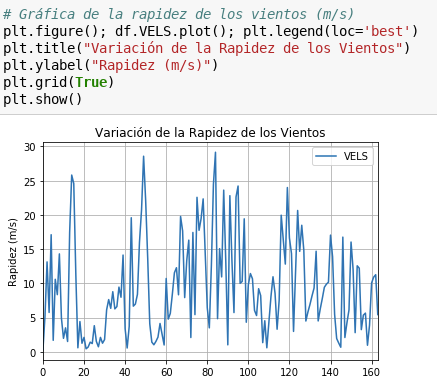
\includegraphics[width=0.5\textwidth]{Rapidez.png}
  \caption{Gráfica de Velocidad de Viento y Velocidad de Rafagas }
  \label{fig:Actividades}
 \end{wrapfigure}
 En la primera parte de la actividad, donde se replicó el contenido del ejemplo brindado por el profesor, se vieron las bases de la programación en python, como cargar a la memoria de trabajo las bibliotecas, leer archivos, mostrar los primeros o últimos datos del archivo, dar estructura a los datos, ver los tipos de datos que el paquete Panda reconoce, combinar columnas, convertir variables, realizar analísis exploratorios de los datos, seleccionar rangos de datos acotando una variable, calcular promedios y hacer gráficas. Todas las acciones se incluyen en la Figura 4, excepto por la sección de gráficas, la cual aparece en la Figura 3. Para realizar las gráficas se utilizó Matplotlib y algunos comandos para especificar el diseño de estas como lo son título de la gráfica, títulos de los ejes, rango de los ejes, forma y color de los datos, 
entre otras.
\begin{center}

    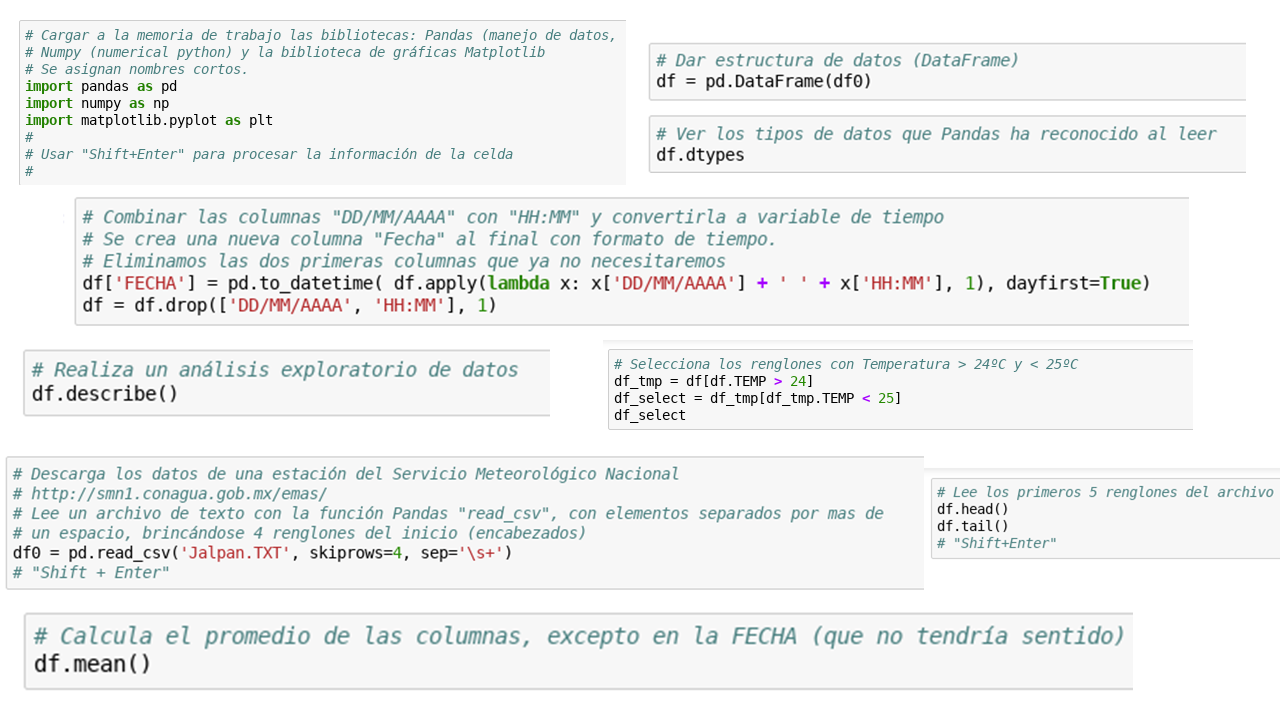
\includegraphics[width=0.99\textwidth]{Acciones.png}

   Figura 4. Actividades realizadas

\end{center}

\subsection{Actividades Adicionales}
\subsubsection {Crear una gráfica que muestre la rapidez de los vientos y la rapidez de las ráfagas, como funciones del tiempo. ¿Cuáles son las horas del día con más viento?.}
\begin{wrapfigure} {l}{0.5\textwidth}
  \centering
  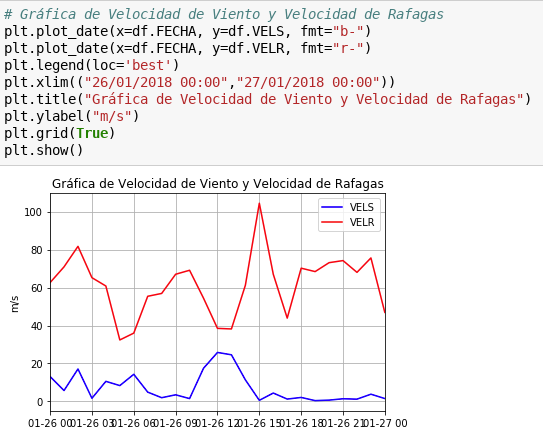
\includegraphics[width=0.45\textwidth]{VelViento.png}
  \label{fig:Actividades}
\end{wrapfigure}


Se puede observar que por la tarde, aproximadamente entre las 16:00-18:00 horas es cuando los vientos tienen mayor rapidez, aun que también por la mañana, a las primeras horas del día se forman picos en las gráficas, lo que quiere decir que también hay un aumento en su rapidez, pero no tan notable como en la tarde.

También se puede observar en la gráfica que los vientos (color azul) siempre tienen mayor velocidad que las ráfags (color rojo).


\subsubsection {Crear una gráfica con la dirección de los vientos como función del tiempo y comentar sobre los vientos dominantes en el sitio de estudio.}
\begin{wrapfigure} {r}{0.4\textwidth}
  \centering
  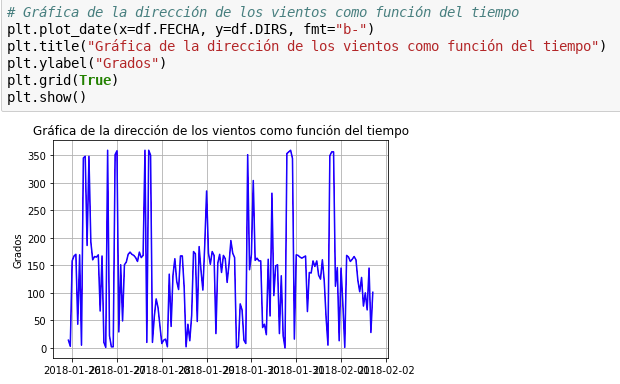
\includegraphics[width=0.4\textwidth]{Direccion.png}
  \label{fig:Actividades}
\end{wrapfigure}

Claramente se nota como la mayoría de los vientos mantienen una dirección constante al rededor de 150\grad, aun que se puede destacar como en ciertos periodos, la dirección cambia brutalmente, aumentando incluso hasta un poco más de los 350\grad. Sin embargo también se ven esos cambios drásticos en disminución, cayendo hasta los 0\grad. 

No hay que olvidar que los datos en la gráfica son los de una semana, por lo que probablemente los cambios de dirección sean debido a las ráfagas de viento que hay en cada diía de la semana.

\subsubsection {Muestre el comportamiento de la Radiación Solar como función del tiempo. ¿Que puedes comentar? }
\begin{wrapfigure} {l}{0.45\textwidth}
  \centering
  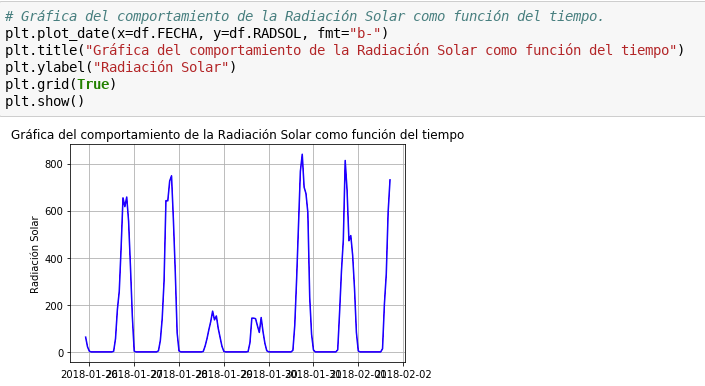
\includegraphics[width=0.35\textwidth]{Radiacion.png}
  \label{fig:Actividades}
\end{wrapfigure}

Al igual que en la gráfica anterior, se pueden observar los "picos", los cuales llegan hasta más de 800, de manera casi constante cada cierto intervalo de tiempo, lo cual también se puede deber a que los datos en el eje x son varios días y que los "picos" se pueden dar a las mismas horas del día.
\subsubsection {¿Cuál es el lapso de temperatura diaria? (Diferencia entre la temperatura máxima y la mínima).}
\begin{wrapfigure} {r}{0.2\textwidth}
  \centering
  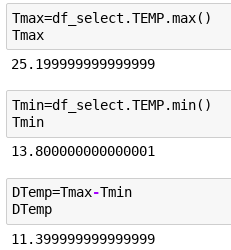
\includegraphics[width=0.2\textwidth]{DifTemp.png}
  \label{fig:Actividades}
\end{wrapfigure}

Para poder contestar esta parte de la actividad, se tuvieron que separar un conjunto de datos, ya que se necesitaba solo un día, esto se logro mediante la entrada que me nuestra debajo del párrafo. Después se buscó el máximo y mínimo del conjunto de datos para verificar que fueran los datos correctos, Para finalizar, se realizó la resta de la temperatura máxima menos la mínima para así poder encontrar la diferencia que se buscaba.
\begin{center}
    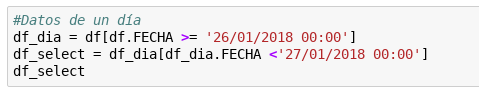
\includegraphics[width=0.5\textwidth]{Datosdia.png}
\end{center}

\subsubsection {¿Puedes comentar sobre la relación entre la temperatura y la humedad relativa?}
\begin{wrapfigure} {l}{0.5\textwidth}
  \centering
  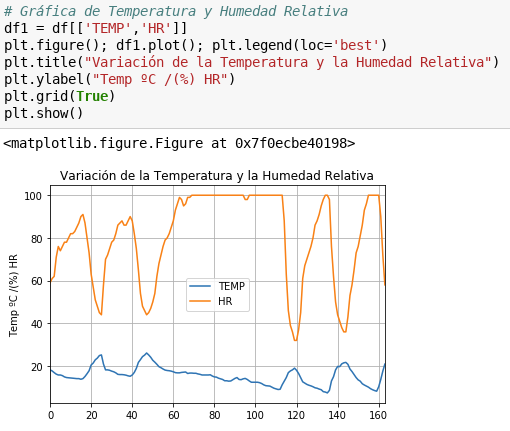
\includegraphics[width=0.4\textwidth]{TempHum.png}
  \label{fig:Actividades}
\end{wrapfigure}
Se nota una clara relación entre ambas, ya que los puntos más altos de la humedad relativa, corresponden a los más bajos de la temperatura, y de igual forma, los puntos más alto de temperatura corresponden a los más bajos de la humedad. 

Incluso en el lapso de tiempo en el que la humedad relativa se mantiene constante, la temperatura también se mantiene sin cambios tan bruscos como los que había presentado antes.

\subsubsection {Realiza el análisis exploratorio de datos, que resuma el sitio estudiado (Usar la función describe() sobre tu data frame.}
\begin{center}
    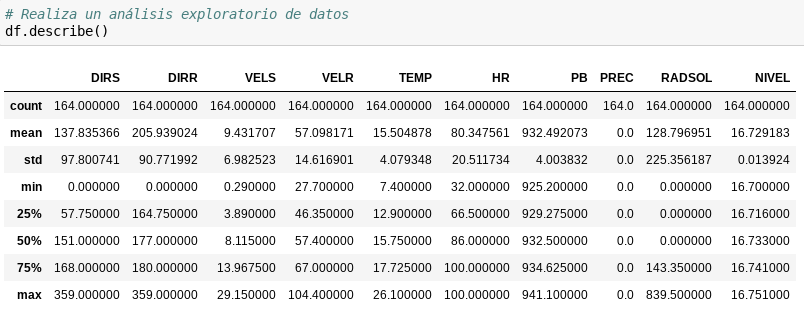
\includegraphics[width=0.85\textwidth]{analisis.png}
\end{center}

\section {Apéndice}
\begin{enumerate}
\item ¿Cuál es tu primera impresión de Jupyter Notebook?
Al inicio me costó trabajo familiarizarme con el entorno, ya que era mi primera vez trabajando en un ambiente así, sin embargo con la practica me acostumbré y me pareció más sencillo de trabajar.
\item ¿Se te dificultó leer código en Python?
No se me dificultó tanto por los comentarios que cada entrada tenía, además de que se utilizan palabras que tienen un significado literal.
\item ¿En base a tu experiencia de programación en Fortran, que te parece el entorno de trabajar en Python?
Me parece un entorno más amigable y sencillo de aprender.
\item A diferencia de Fortran, ahora se producen las gráficas utilizando la biblioteca Matplotlib. ¿Cómo fue tu experiencia?. 
Me pareció excelente como es que se hacían las gráficas en Matplotlib, por que se generaban al momento y se podían personalizar facilmente.
\item En general, ¿qué te pereció el entorno de trabajo en Python? 
Por el momento me parece sencillo de utilizar.
\item ¿Qué opinas de la actividad? ¿Estuvo compleja? ¿Mucho material nuevo? ¿Que le faltó o que le sobró? ¿Qué modificarías para mejorar? 
Me parece un buen comienzo el haber tomado como ejemplo un código ya listo, por que así sé que estoy haciendo y no te pierdes con facilidad. Siento que fue mucha información nueva y sería conveniente hacer como un resuemen de las partes más importantes, algo como resultados sobresalientes.
\item ¿Comentarios adicionales que desees compartir? 
Me hubiera gustado que tuvieramos una sesión más en el laboratorio por la que se perdió el día lunes.
\end{enumerate}

\section{Bibliografía}
\begin{itemize}
\item https://bioinf.comav.upv.es/courses/linux/python/pandas.html
\item https://pandas.pydata.org/pandas-docs/stable/index.html
\item https://es.wikipedia.org/wiki/Python
\item https://www.datacamp.com/community/tutorials/tutorial-jupyter-notebook
\item https://live.osgeo.org/es/quickstart/jupyter_quickstart.html
\subsection{Imágenes}
\item https://commons.wikimedia.org/wiki/File:Python.svg
\item https://gitlab.eurecom.fr/zoe-apps/zapp-jupyter/blob/master/logo.png
\end{itemize}
\end{document}
